\part{Termodinámica}

\vspace*{\fill}

\begin{center}
	\textit{La termodinámica es el estudio de las restricciones a las posibles propiedades de la materia que se derivan de las propiedades de simetría de las leyes fundamentales de la física.}
\end{center}

\vspace*{\fill}

\chapter{Conceptos Básicos}

\paragraph{Propósito: } La termodinámica busca describir sistemas de muchas partículas ($10^{23}$ típicamente). Gases, líquidos, cristales, estrellas, universo, \ldots ,  \underline{sistemas macroscópicos} y en particular, estudiar los procesos de transferencia de energía (trabajo y calor) entre cuerpos macroscópicos\footnote{Más adelante se tratará la parte microscópica con la Mecánica Estadística, poder explicativo y predictivo sobre propiedades macroscópicas de la materia, partiendo de una descripción microscópica.}. 

\begin{itemize}
	\item Definir cantidades físicas, "variables de estado" que caracterizan un sistema macroscópico: $V,T,N,U,\ldots$.
	\item Relacionar estas cantidades entre sí:
		\begin{enumerate}
			\item Válidas para cualquier sistema en equilibrio:
			\begin{enumerate}
				\item Leyes axiomáticas de la termodinámica, como Ley de la Energía, Ley de la Entroía, etc.
			\end{enumerate}
			\item Específicas
			\begin{enumerate}
				\item Por ecuaciones de estado como: fenomenológicas, empíricas, experimentales en la mayoria de los casos.
			\end{enumerate}
		\end{enumerate}
\end{itemize}


Es importante mencionar que la termodinámica clásica macroscópica no puede explicar porqué una ecuación de estado describe un sistema partícular.

\newpage

\section{Sistemas Termodinámicos y Cantidades de Estado}

\begin{enumerate}
	\item Sistema Termodinámico:
	\begin{figure}[H]
		\centering
		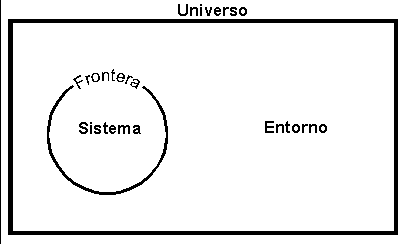
\includegraphics[scale=0.3]{./img/thermodynamicSystem.png}
		\label{thermodynamicSystem}
		\caption{Representación gráfica de las partes de un sistema termodinámico.}
	\end{figure}
	
	\item Tipos de Sistemas: (depende de la frontera)
	\begin{itemize}
		\item Sistemas aislados: No intercambian energía con el entorno. Los sistemas rígidos no pueden intercambiar trabajo y los adiabáticos no pueden intercambiar calor.
		\item Sistemas cerrados: Aquel que intercambia energía y trabajo con su entorno pero la masa permanece constante. Este intercambio de energía puede ser fluctuante aunque la caracterización de estas fluctuaciones no es de interes para la termodinámica.
		\item Sistemas abiertos: Aquel que intercambia tanto energía como materia con su entorno.
	\end{itemize}
	\item Variables de estado: Cualquier cantidad macroscópica que pueda describir el sistema. $E,V,N,T,P,S$, viscocidad $\mu$, composición química, etc. \textbf{no} $\{ \vec{r}_i , \vec{p} _i \}$. 
	\begin{itemize}
		\item Cantidades de estado extensivas: estas son aditivas (dependen de la cantidad de sustancia/moles o masa). Ejemplo: volumen, energía o entropía.
		\item Cantidades de estado intensivas: son independientes de la cantidad de sustancia del sistema, como la densiada, índice de refracción, presión o temperatura.
	\end{itemize}
\end{enumerate}



\section{Equilibrio y Temperatura (Ley Cero de la Termodinámica):}

\begin{enumerate}
	\item Estado de un sistema: Se define por un conjunto particular de \underline{valores} de sus variables termodinámicas.
	\begin{itemize}
		\item Como cada variable describe el sistema como un todo, en general son constantes en el espacio.
		\item Las variables pueden variar (lentamente en el tiempo).
	\end{itemize}
	\item Estado de equilibrio: cada variable tiene un único valor y este valor no cambia en el tiempo.
	\item Procesos cuasi-estáticos y no cuasi-estáticos: un proceso $\equiv$ un cambio de estado. (normalmente un proceso cuasi-estático se toma como un proceso reversible, aquí haremos una distinción). Un proceso no cuasi-estático puede ser una expansión muy rápida de un gas. Mientras que un proceso cuasi-estático puede ser reversible o irreversible como la expansión muy lenta de un gas con un pistón ($\delta V$ es muy pequeña). 
\end{enumerate}

\paragraph{Temperatura y Ley Cero: } La temperatura es una cantidad "desconocida" para la mecánica y electrodinámica, es una cantidad de estado especial para la termodinámica. Esta se define clásicametne mediante un proceso (\dsnote{no hay definición matemática...aún, se verá en la parte de mecánica estadística}). \\
La Ley Cero es una definición de la temperatura: Variable intensiva que es igual en dos sistemas en contacto, en equilibrio sin importar la forma y ubicación de este contacto. \\
Otra definición de la Ley Cero: "Cuando el contacto térmico entre A y B produce que B se caliente y A se enfríe, sin importar donde está este contacto, entonces no hay proceso que pueda calentar A y enfriar B que no induce un trabajo". \\

\" ESTADO DE EQUILIBRIO" $\neq$ \" ESTADO ESTACIONARIO", estar en equilibrio implica ser estado estacionario, pero no al contrario.


\section{Presión, Ecuación de Estado}
\begin{enumerate}
	\item Presión: En términos mecánicos es lo que ya se conoce $F/A$ y en términos microscópicos es la suma de las fuerzas que realizan todas las particulas del sistema sobre $A$.
	\item Ecuación de Estado: Relación entre variables independietes y la temperatura:
		$$ F (X,Y,T) = 0 $$
	\begin{figure}[H]
		\centering
		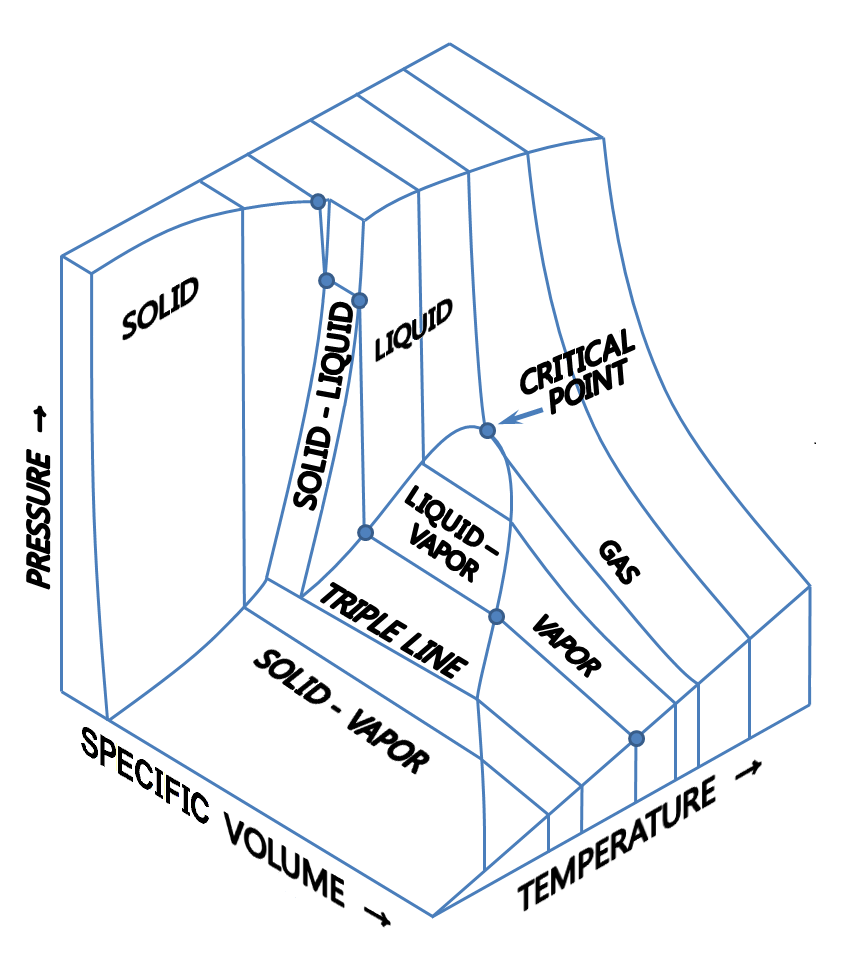
\includegraphics[scale=0.2]{./img/PVT_diagram.png}
		\label{PVT}
		\caption{Diagrama PVT.}
	\end{figure}
	Por ejemplo: Ecuación del gas ideal $pV = nRT$, la ecuación de gas real (expansión del Virial) $pV = Nk_B T + B(T) p + C(T) p^2 + \cdots$, donde $B(T), C(T), \ldots$ son los coeficientes del Virial o la de Van der Waals.
	\item Diferenciales Exactos (e Inexactos): Suponemos una ecuación de estado $z = f(x,y)$. Diferenciación $\dd{f(\vec{r})} = \vec{\nabla} f(\vec{r}) \cdot \dd{\vec{r}}$. $\dd{f}$ es un diferencial total si su integral no depende del contorno y solo de los extremos. Y este es exacto si $f$ es totalmente diferenciable, es decir, se pueden intercambiar las derivadas cruzadas (\dsnote{Básicamente, el teorema de Clairaut}). La implicación que esta tiene en termodinámica son las transformaciones reversibles (que pasan por estados de equilibrio), en estas la ecuación de estado el valor de las variables de estado es independiente del proceso que sigue para llegar a otro estado y esto es válido para cualquier variable de estado.
\end{enumerate}



\chapter{Primera Ley de la Termodinámia}


\section{Trabajo y Calor}
La energía total de un sistema puede variar si recibe (cede) trabajo o calor.

\begin{enumerate}
	\item Trabajo: Sistema sujeto a fuerzas externas. El sistema recibe energía durante una compresión. Con esta idea se tiene la convensión general (\dsnote{Bastante lógico}) $\delta W > 0$ si el sistema recibe trabajo y $\delta W < 0$ si el sistema realiza trabajo. \\
	Caso particular\footnote{Para más ejemplos ver p9 de \href{https://github.com/DSarceno/ExamenPrivado/blob/main/material_\%C3\%BAtil/termodinamica/Notas\%20Boyer.pdf}{Notas Boyer}} procesos cuasi-estáticos, $\dd{\vec{l}}$ es infinitesimal, es decir muy lento, entonces la aceleración del pistón es despresiable $\vec{F} _e + \vec{F}_i = 0$, donde $F_i$ es la fuerza ejercida por el sistema (fuerza interna) entonces $\delta W = - \vec{F} _i \cdot \dd{\vec{l}}$. Como el proceso es cuasi-estático, el sistema está en equilibrio $\leftarrow \, \exists$ presión en el sistema $\vec{F} _i = PA \vu{z}$. Reemplazando en la definición de trabajo $\delta W = -P\dd{V}$ ($P$ cantidad intensiva, $\dd{V}$ cantidad extensiva). \faExclamationTriangle $\,$ Durante el trabajo infinitesimal la presión es aproximadamente constante en el intervalo $[V,V + \dd{V}]$, pero si $\Delta V$ es grande, entonces
		$$ \Delta W = - \int _{V_1} ^{V_2} P(V) \dd{V}. $$
	\item Calor: Es una forma partícular de energía distinta al trabajo, por ejemplo en el calentamiento por entrega de calor no hay un trabajo visible. \\
	\textbf{Experimento de Joule: } Este fue crucial para demostrar la equivalencia entre trabajo mecánico y calor, sentando las bases de la primera Ley de la Termodinámica. 
	\begin{figure}[H]
		\centering
		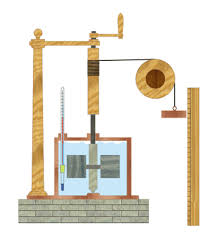
\includegraphics[scale=0.4]{./img/experimentoJoule.jpeg}
		\label{expJoule}
		\caption{Este consiste en un contenedor de agua aislado térmicamente, un sistema de paletas y un peso y una cuerda los cuales pasan por una polea.}
	\end{figure}
	El procedimiento es:
	\begin{enumerate}
		\item Elevación del peso: El peso se levanta a una cierta altura almacenando energía potencial gravitacional.
		\item Al liberar el peso, este desciende, la cuerda hace girar el eje el cual, a su vez, hace girar las paletas.
		\item Las paletas agitan el agua, creando fricción y generando calor.
	\end{enumerate}
	Joule encontró que el aumento de la temperatura del agua estaba directamente relacionado con la cantidad de trabajo mecánico realizado. Específicamente, pudo determinar la equivalencia entre unidades de trabajo (joules) y unidades de calor (calorías). La relación que encontró es aproximadamente $4.184$ joules por caloría. \\
	Joule demostró que el calor podía generarse mediante trabajo mecánico y viceversa, consolidado el concepto moderno de energía. \\
	Además podemos concluir que $\delta Q$ y $\delta W$ no son cantidades de estado, dependen del proceso, del camino ($Q$ y $W$ no son diferenciales exactos).
\end{enumerate}

\subsection{Naturaleza del Calor}
\" Energá distribuída de manera desordenada entre partículas. \" Es mucho más fácil convertir trabajo en calor que al revés. \\
Convensión: Misma que para el trabajo: $\delta Q = \delta Q_{\text{entorno} \leftarrow \text{ sistema}}$
\begin{itemize}
	\item $\delta Q > 0$ para un sistema que recibe calor del entorno.
	\item $\delta Q < 0$ para un sistema que cede calor al entorno.
\end{itemize}

\section{Energía Interna y Primera Ley}

\begin{enumerate}
	\item Energía interna: (definición microscópica) $U$ esta es la energía total del sistema, en el sentido mecánico-newtoniano, con  $N$ partículas
		$$ U = \sum _{i=1} ^N \frac{1}{2} m_i v_i ^2 + \sum _{i=1} ^N \sum _{j > i} ^N V(\vec{r}_i ,\vec{r}_j) + \sum _{i=1} ^N \vec{F} _e ^i \cdot \vec{r}_i . $$
	Donde se tiene la energía cinética, la potencial y las fuerzas externas. En general es imposible calcular esta energía y tampoco es el propósito de este curso. \dsnote{como siempre, a esperar a mecánica estadística} \\
	(definición macroscópica): Es equivalente a la definición de microscópica si $N\to \infty$. Cantidad de estado que varía cuando el sistema recibe trabajo o calor y que tiene dimensión de energía.
	\item Primera Ley de la Termodinámica: Conservación de la energía $U$ (\dsnote{Es básicamente una conservación de la energía, como se ve en física 1, pero con esteroides}) 
		$$ \dd{U} = \delta Q + \delta W. $$
	Formas estándares de la primera ley:
	\begin{itemize}
		\item Sistemas aislados: $\dd{U} = 0$
		\item Sistemas cerrados: $\dd{U} = \delta Q - P\dd{V}$
		\item Sistemas abiertos: $\dd{U} = \delta Q - P\dd{V} + \mu \dd{N}$\footnote{En transformaciones cuasi-estáticas}.
	\end{itemize}
\end{enumerate}


\section{Implicaciones de la Primera Ley}

\begin{enumerate}
	\item La energía interna es una variable de estado y un diferencial exacto:
		$$ \dd{U} = \qty(\pdv{U}{T})_{V,N} \dd{T} + \qty(\pdv{U}{V})_{T,N} \dd{V} + \qty(\pdv{U}{N})_{V,T} \dd{N}. $$
		Y $f(V,T,N)$ se conoce como la ecuación de estado.
	\item Procesos Cíclicos: Son procesos de partícular interés. En estos procesos $U_f = U_o$ o, en otras palabras
		$$ \oint \dd{U} = 0, $$
	esto implica $\Delta W + \Delta Q = 0 \qquad \Delta W = - \Delta Q \neq 0$, en esto se tienen dos casos importantes
		\begin{itemize}
			\item Caso $\Delta W < 0$: \underline{motor}, fuente de calor en el entorno, pero necesitamos $\Delta Q > 0$.
			\item Caso $\Delta Q < 0$: \underline{refrigerador}, trabajo sobre el sistema, pero se necesita $\Delta W > 0$.
		\end{itemize}
\end{enumerate}


\section{Capacidad Calorífica}

Se define como $\delta Q = c \dd{T}$, un incremento o decremento de temperatura, donde la constante $c$ es la capacidad calorífica. Recordemos que $\dd{U} = \delta Q - P\dd{V}$ para un sistema cerrado sin fuerzas externas.

		$$ C_V = \qty(\frac{\delta Q}{\delta T}) _V, \quad \text{Volumen constante,} $$
		$$ C_P = \qty(\frac{\delta Q}{\delta T}) _P, \quad \text{presión constante,} $$

	y como consecuencia de la primera ley: $V=\text{cte}$ entonces $\dd{U} = \delta Q$ por ende $C_V = \qty(\dv{U}{T})_V$. $C_V$ y $C_P$ son cantidades extensivas, en algunos libros $C_v = \frac{1}{N} \qty(\dv{U}{T})_V$ capacidad por partícula o por mol (en este caso sería una cantidad intensiva).
	
\paragraph{Gas Ideal} se tienen dos casos, para un gas monoatómico y diatómico
	$$ \text{Monoatómico} \qquad U = \frac{3}{2} N k_B T, $$
	$$ \text{Diatómico} \qquad U = \frac{5}{2} N k_B T. $$

Para todo material en equilibrio se tiene la siguiente relación entre $C_V$ y $C_P$. Para ello se considerará $N=cte$ (sistema cerrado), como variables se tienen $P,V,T$; sin embargo, $f(P,V,T) = 0$ es la ecuación de estado de equilibrio. Por ello se toman dos variables independientes $U = U(P,V) = U(P,T) = U(V,T)$. Además se tienen dos maneras de escribir el diferencial de energía interna: la primera ley y el diferencial total. Con esto:
	$$ \delta Q - p\dd{V} = \qty(\pdv{U}{T})_{V} \dd{T} + \qty(\pdv{U}{V})_{T} \dd{V} $$
	$$ \delta Q = \qty(\pdv{U}{T})_{V} \dd{T} + \qty[p + \qty(\pdv{U}{V})_{T}] \dd{V} $$
dividiendo entre $\dd{T}$ se tiene
	$$ C_P = \underbrace{\qty(\pdv{U}{T})_{V}}_{C_V} + \qty[p + \qty(\pdv{U}{V})_{T}] \qty(\frac{\delta Q}{\delta T}) _P $$
	$$ \boxed{ C_P - C_V = \qty[p + \qty(\pdv{U}{V})_{T}] \qty(\frac{\delta Q}{\delta T}) _P. } $$
	
	Esta siempre es positiva. Para un gas ideal $\qty(\pdv{U}{V})_{T} = 0$, $p = \frac{Nk_B T}{V}$, $\qty(\frac{\delta Q}{\delta T}) _P = \frac{V}{T}$.
	$$ \boxed{ C_p - C_V = Nk_B } $$
	


\section{Procesos Adiabáticos}
Es aquel proceso reversible en un sistema térmicamente aislado, por lo que no existe un intercambio de calor entre él y el entorno $\delta Q = 0$. Por lo que $\dd{U} = -p\dd{V}$, y en un gas ideal $\dd{U} = \qty(\pdv{U}{T})_V \dd{T} = C_V \dd{T}.$ Lo que implica que
	$$ \frac{\dd{T}}{T} = \frac{C_p - C_V}{C_V} \frac{\dd{V}}{V}. $$
	
Donde $\frac{C_P}{C_V} = \gamma$, número adimensional. Integrando \dsnote{Y haciendo calculito del kinder, como diría Damián} se tienen las siguientes equivalencias
	$$ \boxed{ T V ^{\gamma - 1} = PV^\gamma = T^\gamma P^{1 - \gamma} = \text{cte}. } $$
	
\subsection{Trabajo Adiabático}


Teniendo $\delta W = -p\dd{V}$, las equivalencias anteriores y nuevamente calculito del kinder y se llegamos a lo siguiente
	$$ \boxed{ \Delta W = \frac{1}{\gamma - 1} \qty[P_1 V_1 - P_o V_o] = \frac{Nk_B}{\gamma - 1} [T_1 - T_o] = C_v [T_1 - T_o]. } $$
	
Es claro que se puede llegar a este resultado directamente desde la primera ley.



\chapter{Procesos Cíclicos}

\section{Tipos de Procesos}
El primer tipo es aquel que tiene una variable de estado constante: isotérmicos, isocóricos, isobáricos y adiabáticos \dsnote{el nombre es bastante claro con lo que implica cada proceso}. 


\subsection{Procesos Reversibles e Irreversibles}
Un proceso se dice reversible cuando estados sucesivos del mismo procesos difieren infinitesimalmente de estados de equilibrio. Dado esto, existen procesos reversibles termodinámicamente, los cuales cumplen con dos condiciones: ser cuasi-estático y un proceso no disipativo.

\section{Ciclo de Carnot}
El \textbf{ciclo de Carnot} se produce en un equipo o máquina cuando trabaja absorbiendo una cantidad de calor $Q_1$ de una fuente de mayor temperatura y cendiendo una cantidad de calor $Q_2$ a la de menor temperatura produciendo un trabajo sobre el exterior.

	\begin{figure}[H]
		\centering
		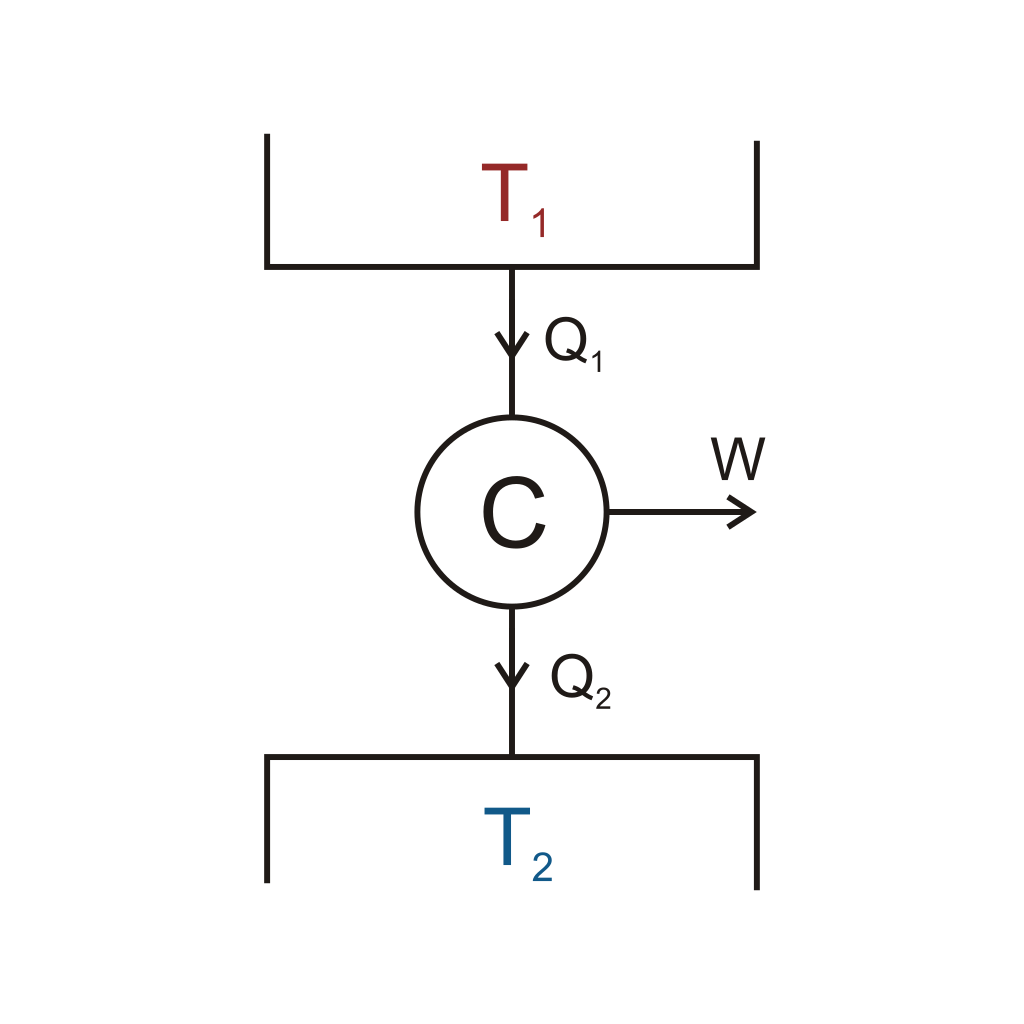
\includegraphics[scale=0.1]{./img/carnot.png}
		\label{carnot}
		\caption{Esquema de una máquina de Carnot.}
	\end{figure}

El rendimiento del ciclo está definido por
	$$ \eta = 1 - \frac{Q_2}{Q_1}. $$
Y, como se verá más adelante, es el mayor producido por cualquier máquina que funcione cíclicamente entre las mismas fuentes de temperatura. \\
Como todos los procesos que tienen lugar en el ciclo ideal son reversibles, el ciclo puede invertirse y la máquina absorbería calor de la fuente fría y cedería calor a la fuente caliente, teniendo que suministrar trabajo a la máquina. Si el objetivo de esta máquina es extraer calor de la fuente fría (para mantenerla fría) se denomina máquina frigorífica, y si es ceder calor a la fuente caliente, bomba de calor. \\

El ciclo de Carnot\footnote{Ver \href{https://es.wikipedia.org/wiki/Ciclo_de_Carnot}{wikipeeeediaaa} para la explicación detallada de cada paso.} consta de cuatro etapas: dos procesos isotermos y dos adiabáticos, como se muestra en el siguiente diagrama P-V

	\begin{figure}[H]
		\centering
		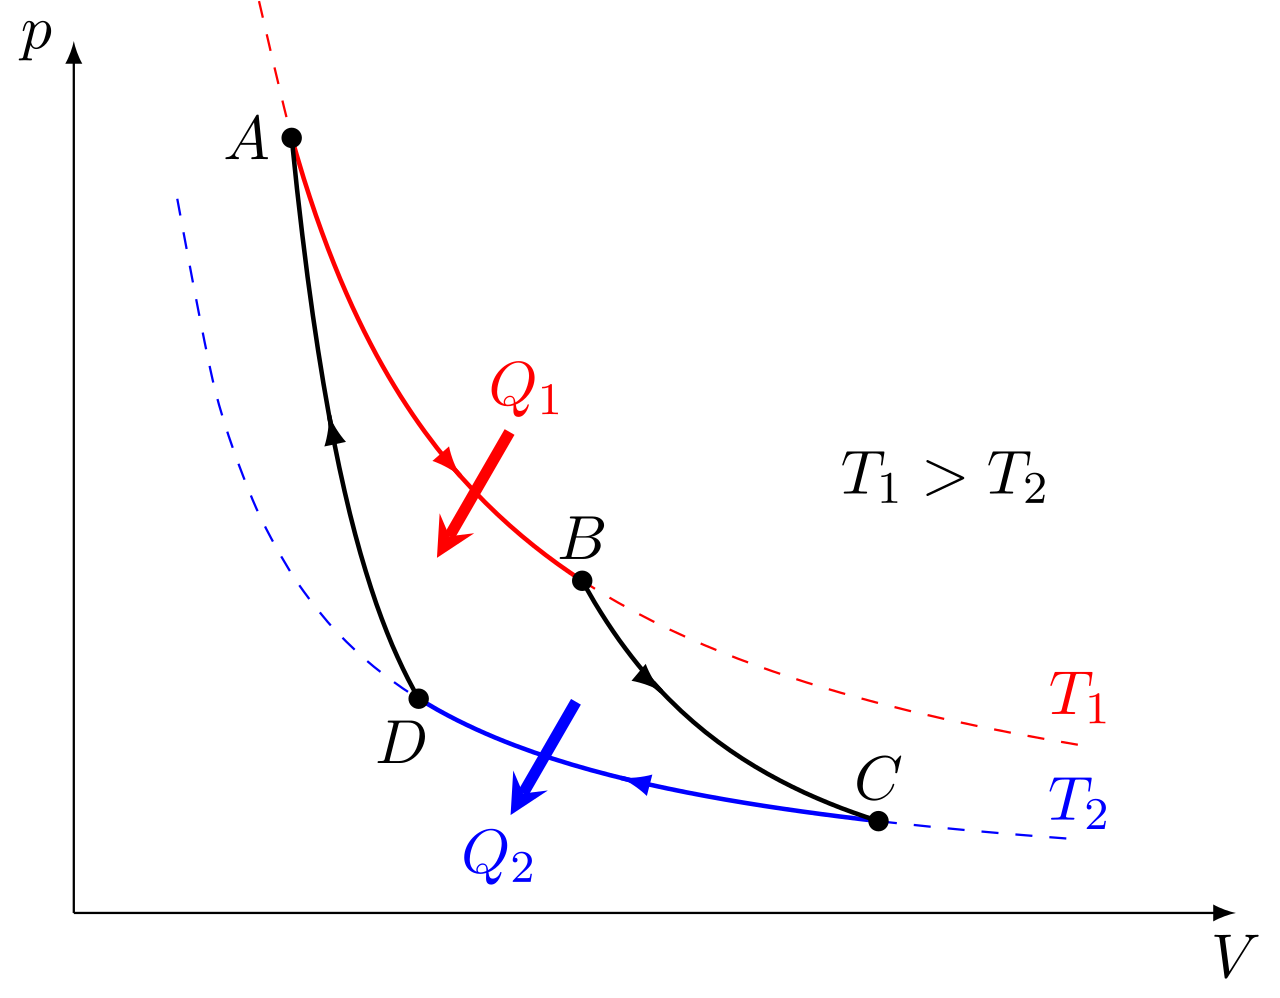
\includegraphics[scale=0.15]{./img/PV_Ciclo_de_Carnot.png}
		\label{clapeyronCarnot}
		\caption{Ciclo de carnot en el diagrama de Clapeyron.}
	\end{figure}

\begin{itemize}
	\item AB: Expansión isoterma;
	\item BC: Expansión adiabática;
	\item CD: Comprensión isoterma;
	\item DA: Comprensión adiabática.
\end{itemize}

\subsection{Teoremas de Carnot}

\begin{enumerate}
	\item No puede existir una máquina térmica que funcionando entre dos fuentes térmicas dadas tenga mayor rendimiento que una de Carnot que funcione entre esas mismas fuentes térmicas.
	\item Dos máquinas reversibles operando entre las mismas fuentes térmicas tienen el mismo rendimiento.
\end{enumerate}



\chapter{Segunda Ley de la Termodinámica}

\section{Kelvin-Planck}
Es imposible construir un motor que opere en ciclos y extraiga calor de una fuente que convierta el calor extraído exclusivamente en trabajo.

\section{Clauius}
Es imposible construir un frigorífico que, operando en un ciclo, transferencia completamente el calor de una fuente de menor temperatura a una fuente de temperatura mayor.

\dsnote{Raras tus formulaciones pue.}

\section{La que te venden los divulgadores}
\textit{La cantidad de entropía del universo tiende a incrementarse en el tiempo.} Este principio establece la irreversibilidad de los procesos físicos, especialmente durante el intercambio de calor.

\section{Reversibilidad e Irreversibilidad}
Un proceso reversible es un proceso que realiza de tal forma que el sistema y su entorno pueden regresara su sestados iniciales sin producir ningún cambio en el resto del universo. (\dsnote{Si, es otra forma de redactar la reversibilidad.})



\chapter{Entropía}

La entropía es posiblemente el más importante e insuficientemente conocido concepto en fisiología. Es una magnitud física que permite determinar la parte de la energía que no puede utilizarse para producir trabajo y está ligada con el grado de desorden de un sistema.


\section{Definición de Entropía}
Ya se introdujo la integral $\oint \dbar Q / T = 0$. Esto implica que la integral
	$$ \int _A ^B \frac{\dbar Q}{T} $$
es independiente del camino; por ende, se define entropía como el diferencial exacto 
	$$ \boxed{ \dd{S} = \frac{\dbar Q}{T}, } $$
tal que
	$$ S(B) - S(A) = \int _A ^B \frac{\dbar Q}{T}, $$
y $S$ es una función de estado. Para un proceso adiabático se tiene que $\dbar Q = 0$. Por eso un proceso adiabático no presenta cambios en la entropía (los procesos adiabáticos también son llamados isoentrópicos).


\section{Cambios Irreversibles}
Ya se tiene la definición de entropía en términos de cambios reversiles. Dado que $S$ es una función de estado
	$$ \oint \frac{\dbar Q_{rev}}{T} = 0. $$
Entonces
	$$ \dd{S} = \frac{\dbar Q_{rev}}{T} \geq \frac{\dbar Q}{T}. $$
Consideremos un sistema térmicamente aislado $\dbar Q = 0$; por lo tanto $\dbar S \geq 0$. \\

La entropía solo puede mantenerse igual (cambios reversibles) o aumentar (cambios irreversibles). Tomando al universo como un sistema térmicamente aislado.


\section{Regresando a la Primera Ley}
Ahora podermos mostrar una forma más elegante y útil de la 1ra ley
	$$ \dd{U} = \dbar Q + \dbar W, $$
pero $\dbar Q = T\dd{S}$ y $\dbar W = -p\dd{V}$.
	$$ \dd{U} = T\dd{S} - p\dd{V} $$
en esto se asume un proceso reversible. Pero para uno irreversible se tiene que $\dbar Q \leq T\dd{S}$ y $\dbar W \geq -\dd{V}$. Lo que se nivela y siempre se llega a lo visto para procesos reversibles. \\

$S,V$ son extensivas y $T,p$ son intensivas\footnote{Esto funciona por el teorema recíproco y por el teorema de reciprocidad: $\qty(\pdv{x}{y})_z \qty(\pdv{y}{z})_x \qty(\pdv{z}{x})_y = -1$.}
	$$ \dd{U} = \underbrace{\qty(\pdv{U}{S})_V}_{T} \dd{S} + \underbrace{\qty(\pdv{U}{V})_S}_{-p} \dd{V}. $$
	
\dsnote{Ahora toca profanar la matemática.}

	$$ \frac{p}{T} = \qty(\pdv{S}{V})_U. $$
	


{\Large \textbf{Resumen}} \\
\begin{itemize}
	\item $\dd{U} = \dbar Q + \dbar W$ siempre es cierto
	\item $\dbar Q = T\dd{S}$ reversibles
	\item $\dbar W = -p\dd{V}$ reversibles
	\item $\dbar W \geq -p\dd{V}$ y $\dbar Q \leq T\dd{S}$ irreversibles.
\end{itemize}


\section{Expansión de Joule (Expansión Libre)}
Es un proceso irreversible en el cual un gas se expande en un recipiente vacío y aislado. Los gases experimentan un cambio de temperatura durante la expansión libre.


	\begin{figure}[H]
		\centering
		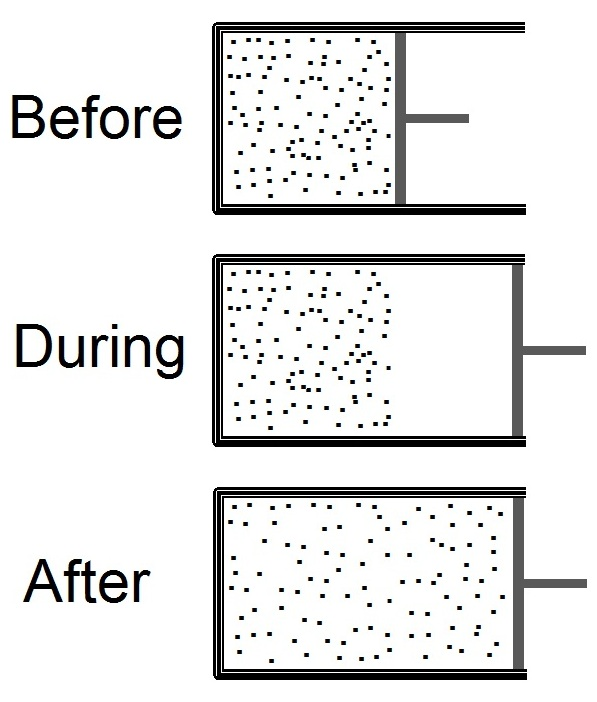
\includegraphics[scale=0.25]{./img/expansionJoule.jpg}
		\label{expansionJoule}
		\caption{También se puede lograr moviendo el pistón hacia fuera más rápido que los átomos del gas.}
	\end{figure}
	
Durante la expansión libre, ningún trabajo es realizado por el gas. El bas pasa a través de los estados que no están en equilibrio termodinámico antes de llegar a su estado fina, lo que implica que no se pueden definir parámetros termodinámicos como valores del gas en su conjunto. \\

Una expansión libre se consigue típicamente mediante la apertura de una llave de paso que permite que el gas se expanda en un vacío. Aunque sería difícil de lograr en la realidad, es instructivo imaginar una expansión libre causada por un pistón en movimiento más rápido que prácticamente cualquier átomo. Ningún trabajo se hace porque no hay presión sobre el pistón. Sin energía térmica que sale o entra en el pistón. Sin embargo, hay un cambio de entropía.

	$$ \Delta S = \int _i ^f \dd{S} = \int _{V_o} ^{2V_o} \frac{p\dd{V}}{T} = \int _{V_o} ^{2V_o} \frac{R\dd{V}}{V} = R\ln{2}. $$



	\begin{figure}[H]
		\centering
		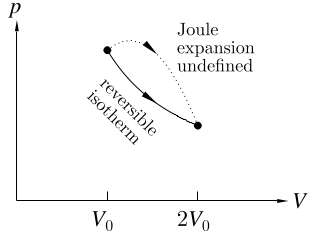
\includegraphics[scale=0.35]{./img/expansionJoule2.png}
		\label{expansionJoule}
	\end{figure}

Luego de que suceda la expansión de Joule, solo se puede poner el gas a la izquierda comprimiendolo. El método que involucra la menor cantidad de trabajo es una compresión isotérmica, cuyo trabajo para 1 mol de gas es
	$$ \Delta W = - \int _{2V_o} ^{V_o} p\dd{V} = - \int _{2V_o} ^{V_o} \frac{RT}{V} \dd{V} = RT\ln{2} = T \Delta S_{gas}. $$
El incremento de entropía en una expansión de Joule es $\Delta W/T$.


{\Large \textbf{Paradoja?}} \\
\begin{itemize}
	\item En la expansión de Joule, el sistema es aislado térmicamente, por lo que no hay flujo/intercambio de calor: $\Delta Q = 0$.
	\item No hay trabajo realizado: $\Delta W = 0$.
	\item Por ello $\Delta U = 0$ (para un gas ideal, $\Delta T = 0$).
	\item Pero si $\Delta Q = 0$, esto implica que $\Delta S = \Delta Q/T = 0$?
\end{itemize}
 El razonamiento anterior es correcto hasta la última parte: la respuesta a la ultima preguna es \textbf{NO!} La ecuación $\dbar Q = T\dd{S}$ es cierto solamente para procesos reversibles. En general $\dbar Q \leq T\dd{S}$, y se tiene $\Delta Q = 0$ y $\Delta S = R \ln{2}$, entonces se tiene que $\Delta Q \leq T \dd{S}$.









































































%%%%%%%%%%%%%%%%%%%%%%%